\documentclass[12pt]{article}

\usepackage{fullpage}
\usepackage{graphicx}
\usepackage{amssymb}
\usepackage{amsmath}
\usepackage[none]{hyphenat}
\usepackage{parskip}
\usepackage[spanish]{babel}
\usepackage[utf8]{inputenc}
\usepackage{hyperref}
\usepackage{fancyhdr}
\usepackage{tasks}
\usepackage{mdframed}
\usepackage{xcolor}
\usepackage{pgfplots}
\usepackage[makeroom]{cancel}
\usepackage{multicol}
\usepackage[shortlabels]{enumitem}
\usepackage{stackrel}
\usepackage{tkz-tab}
\usepackage{xpatch}
\usepackage{tkz-euclide}
\usetkzobj{all}
\usepackage{tabto}
\xpatchcmd{\tkzTabLine}{$0$}{$\bullet$}{}{}

\setlength{\headheight}{10pt}
\setlength{\headsep}{10pt}
\pagestyle{fancy}
\rhead{\ayudantia \ - \alumno}
\tikzset{t style/.style={style=solid}}

\newcommand*{\mybox}[2]{\colorbox{#1!30}{\parbox{.98\linewidth}{#2}}}

\newenvironment{solucion}
{\begin{mdframed}[backgroundcolor=black!10]
		{\bf Solución:}\\
	}
	{
	\end{mdframed}
}

\newenvironment{alternativas}[1]
{\begin{multicols}{#1}
		\begin{enumerate}[a)]
		}
		{
		\end{enumerate}
	\end{multicols}
}

\newenvironment{preguntas}
{\begin{enumerate}\itemsep12pt
	}
	{
	\end{enumerate}
}

\newcommand{\ayudantia}{{\sc Ayudantía 6}}
\newcommand{\tituloayu}{Funciones de varias variables}
\newcommand{\fecha}{17 de septiembre de 2019}
\newcommand{\sigla}{MAT1620}
\newcommand{\nombre}{Cálculo II}
\newcommand{\profesor}{Wolfgang Rivera}
\newcommand{\ano}{2019}
\newcommand{\semestre}{2}
\newcommand{\mail}{mat1620@ifcastaneda.cl}
\newcommand{\alumno}{Ignacio Castañeda - \mail}

\newcommand{\ev}{\Big|}
\newcommand{\ra}{\rightarrow}
\newcommand{\lra}{\leftrightarrow}
\newcommand{\N}{\mathbb{N}}
\newcommand{\R}{\mathbb{R}}
\newcommand{\Exp}[1]{\mathcal{E}_{#1}}
\newcommand{\List}[1]{\mathcal{L}_{#1}}
\newcommand{\EN}{\Exp{\N}}
\newcommand{\LN}{\List{\N}}
\newcommand{\comment}[1]{}
\newcommand{\lb}{\\~\\}
\newcommand{\eop}{_{\square}}
\newcommand{\hsig}{\hat{\sigma}}
\newcommand{\widesim}[2][1.5]{
	\mathrel{\overset{#2}{\scalebox{#1}[1]{$\sim$}}}
}
\newcommand{\wsim}{\widesim{}}
\newcommand{\lh}{\stackrel{L'H}{=}}

\begin{document}
\thispagestyle{empty}

\begin{minipage}{2cm}
	
\includegraphics[width=2cm]{../../../../img/logo.pdf}
	\vspace{0.5cm}
\end{minipage}
\begin{minipage}{\linewidth}
	\begin{tabular}{lrl}
		{\scriptsize\sc Pontificia Universidad Catolica de Chile} & \hspace*{0.7in}Curso: &
		\sigla  - \nombre\\
		{\sc Facultad de Matemáticas}&
		Profesor: & \profesor \\
		{\sc Semestre \ano-\semestre} & Ayudante: & {Ignacio Castañeda}\\
		& {Mail:} & \texttt{\mail}
	\end{tabular}
\end{minipage}

\vspace{-10mm}
\begin{center}
	{\LARGE\bf \ayudantia}\\
	\vspace{0.1cm}
	{\tituloayu}\\
	\vspace{0.1cm}
	\fecha\\
	\vspace{0.4cm}
\end{center}

\begin{preguntas}
\item Determina el dominio de las siguientes funciones
\begin{tasks}(2)
\task $f(x, y) = \sqrt[]{x+y} + \ln(x^2+y^2)$
\task $f(x,y) = \dfrac{x+y}{x^2-y^2}$
\task $f(x,y,z) = ln(z+y) - \dfrac{1}{x^2 +z^2}$
\task $f(x,y,z) = \sqrt[]{\ln(x+y+z)}$
\end{tasks}
\begin{solucion}

\begin{enumerate}[a)]
\item $f(x, y) = \sqrt[]{x+y} + \ln(x^2+y^2)$\\
\\
Notemos que hay dos restricciones que se deben cumplir. La raiz no debe tener argumento negativo y el logaritmo debe tener argumento positivo. Luego, el dominio de la función es
$$Dom(f) = \{(x,y) \in \R^2 | x + y \geq 0 \wedge x^2 + y^2 > 0\}
\item $f(x,y) = \dfrac{x+y}{x^2-y^2}$\\
\\
En este caso nuestra unica restricción es que el denominador sea distinto de 0, por lo que debe ocurrir que
$$x^2 - y^2 \neq 0 \ra x \neq y \wedge x \neq -y$$
Por lo que el dominio será
$$Dom(f) = \{(x,y) \in \R^2 | x \neq y \wedge x \neq -y\}$$
\item $f(x,y,z) = ln(z+y) - \dfrac{1}{x^2 +z^2}$\\
\\
Nuevamente debemos hacer que el logaritmo sea positivo y el denominador distinto de 0. Para el logaritmo es trivial pero notemos que el denominador solo podrá ser 0 si $x$ y $z$ son 0. \\

Luego,
$$Dom(f) = \{(x,y,z) \in \R^3 | z + y > 0 \wedge (x,y,z) \neq (0,y,0) \forall y \in \R \}$$
\item $f(x,y,z) = \sqrt[]{\ln(x+y+z)}$\\
\\
En este caso, notemos que no solamente el argumento del logaritmo debe ser positivo, sino que tambien el resultado de este debe ser no negativo, ya que esto irá dentro de la raiz.\\

Esto es,
$$\ln(x+y+z) \geq 0 \ra x + y + z \geq 1$$
Finalmente,
$$Dom(f) = \{(x,y,z) \in \R^3 | x + y + z \geq 1 \}$$
\end{enumerate}
\end{solucion}
\item Determina el recorrido de las siguientes funciones
\begin{tasks}(2)
\task $f(x,y) = x^2 + y^2 + 3$
\task $f(x,y,z) = \ln(\sqrt[]{x^2+y^2+4}) + z^2$
\end{tasks}
\begin{solucion}

\begin{enumerate}[a)]
\item $f(x,y) = x^2 + y^2 + 3$\\
\\
Notemos que los primeros dos terminos será siempre positivos y el menor valor que pueden tomar es 0.\\

Luego, el recorrido será
$$Rec(f) = [3, \infty)$$
\item $f(x,y,z) = \ln(\sqrt[]{x^2+y^2+4}) + z^2$\\
\\
El valor de la raiz que se encuentra dentro del logaritmo será a lo menos 2, ya que los primeros dos terminos pueden tomar mínimo 0 y luego quedará el 4. Luego, el mínimo valor del logaritmo será $\ln(2)$.\\
\\
Por otro lado, $z^2$ será a lo menos 0, con lo que el recorrido que nos queda es
$$Rec(f) = [\ln(2), \infty)$$
\end{enumerate}
\end{solucion}
\item Grafique las curvas de nivel de la función 
	$$ f(x,y) = \sqrt[]{9-x^2-y^2}$$
	para $k=0,1,2,3$
\begin{solucion}

		Las curvas de nivel de la función corresponden a
		$$\sqrt[]{9-x^2-y^2} = k \ra 9-x^2-y^2 = k^2 \ra x^2+y^2 = 9-k^2$$
		Notemos que esto corresponde a circunferencias de radio $\sqrt[]{9-k^2}$.
		
		Reemplazando con los valores de $k$ indicados, las curvas de nivel a graficar son
		$$k = 0 \ra x^2+y^2 = 9$$
		$$k = 1 \ra x^2+y^2 = 8$$
		$$k = 2 \ra x^2+y^2 = 5$$
		$$k = 3 \ra x^2+y^2 = 0$$
		Graficando,
		
		\begin{center}
			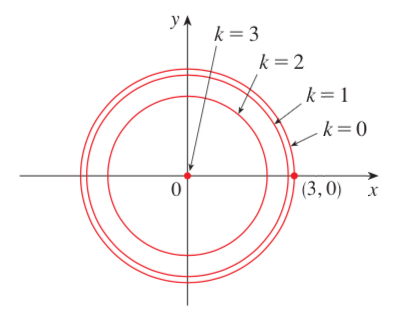
\includegraphics[scale=0.4]{../../../../img/curvasdenivel}			
		\end{center}
\end{solucion}
\end{preguntas}
\end{document}